\section{Process Mining Applications in Industrial Control Systems}

The integration of process mining techniques into industrial control systems represents a significant advancement in the field of cyber-physical systems, offering novel approaches to system modeling, verification, and control generation. Process mining, traditionally applied in business process management, has evolved to address the unique challenges of industrial automation, providing data-driven methods for understanding complex system behaviors and generating formal models from recorded event traces.

This chapter presents three complementary approaches that demonstrate the versatility and effectiveness of process mining in industrial control systems. The first approach focuses on process model extraction and conformance checking for anomaly detection and system monitoring. The second approach introduces an interactive learning methodology for automatic controller generation through simulation-based event recording. The third approach extends these capabilities to automatic plant model generation and real-time monitoring for formal verification.

These methodologies collectively address critical challenges in modern industrial automation: the need for automated system understanding, the complexity of controller development, and the requirement for formal verification in safety-critical applications. By leveraging process mining algorithms and the IEC 61499 standard, these approaches provide systematic methods for transforming recorded behavioral traces into formal models that can be used for system analysis, control generation, and verification.

\begin{figure*}[!t]
	\centering
	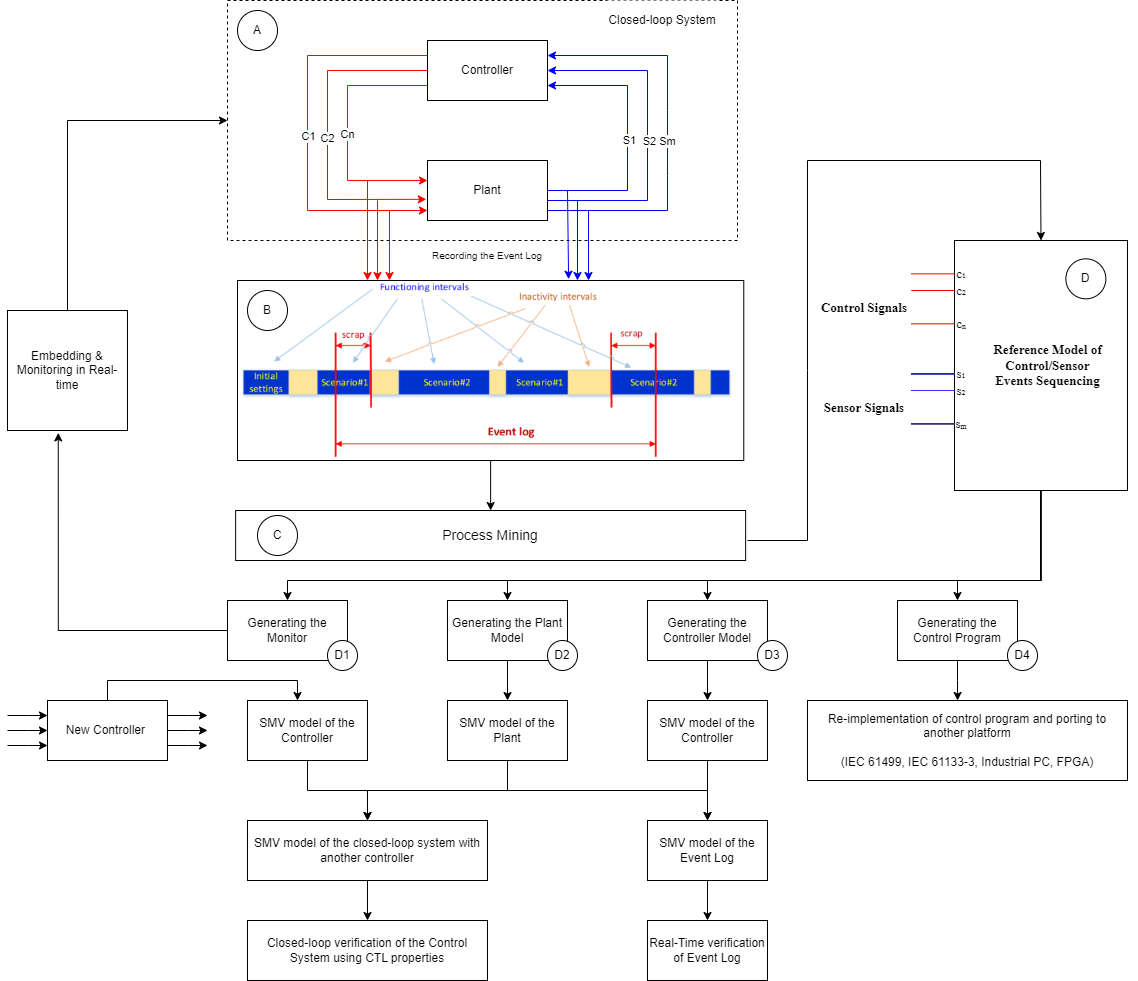
\includegraphics[width=0.9\textwidth]{chapters/images/chapter4/workflow1.png}
	\caption{Workflow and use cases for process mining applications in industrial control systems. The workflow illustrates the transformation from recorded event logs to various applications including monitor generation (D1), plant model generation (D2), control model generation (D3), and control program generation (D4).}
	\label{workflowUsecase}
\end{figure*}

Figure \ref{workflowUsecase} illustrates the comprehensive workflow and potential use cases enabled by process mining in industrial control systems. Initially, signals from distributed control systems are recorded to construct behavioral models using process mining techniques. These models then serve as the basis for generating monitors for real-time error detection, plant models for formal verification, control models for automatic controller generation, and control programs for system implementation. This integrated approach provides a systematic framework for addressing the complex requirements of modern industrial automation systems.

\section{Process Model Extraction and Conformance Analysis}

The application of process mining techniques in industrial control systems begins with the fundamental challenge of understanding system behavior through recorded event logs. This approach leverages the inherent data-rich nature of modern automation systems to extract meaningful process models that can be used for system analysis, anomaly detection, and performance optimization.

\subsection{Process Mining Fundamentals in Industrial Contexts}

Process mining in industrial control systems differs fundamentally from its business process applications by focusing on the temporal and causal relationships between sensor and actuator signals rather than human activities. The core principle involves analyzing event logs that capture the sequence of control and sensor events occurring during system operation, then applying discovery algorithms to extract formal process models that represent the system's behavioral patterns.

The process mining workflow in industrial contexts typically involves three main phases: process discovery, conformance checking, and process enhancement. Process discovery algorithms analyze event logs to generate process models in various formalisms, most commonly Petri nets, which provide a mathematical foundation for representing concurrent and sequential behaviors. Conformance checking compares observed behavior against expected models to identify deviations, while process enhancement focuses on improving existing models based on new observations.



The selection of appropriate process discovery algorithms is crucial for effective model extraction. Alpha algorithm, as a representative of abstraction-based methods, generates models by analyzing ordering relations between events in the log. This algorithm creates dependency graphs based on the sequence of events, making it suitable for systems with well-defined, deterministic behaviors. However, its sensitivity to noise in event logs can lead to overly complex models when dealing with systems that exhibit significant variability.

Heuristic-based algorithms, such as the fuzzy miner, offer an alternative approach that considers the frequency of event occurrences. These algorithms generate models based on the relative importance of activities and the strength of their relationships, making them more robust to noise and better suited for systems with complex, variable behaviors. The fuzzy miner, in particular, provides interactive representations that help understand system behavior in complex logs, though it may be more challenging to convert to other process modeling languages.

\begin{figure}[!t]
	\centering
	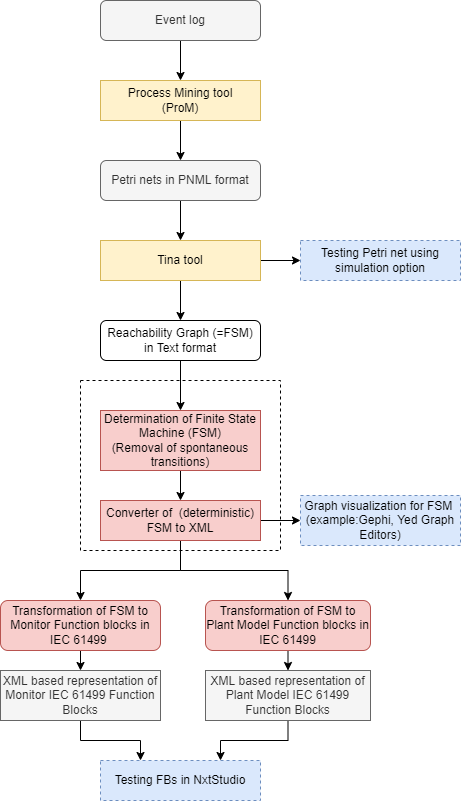
\includegraphics[width=0.4\textwidth]{chapters/images/chapter4/Methodology.png}
	\caption{Tool chain and data flow for generating FSMs from Event Logs and their implementation in the form of IEC 61499 FBs. The process involves preprocessing event logs, applying process discovery algorithms, generating Petri nets, decomposing into state machine components, and finally implementing as IEC 61499 function blocks.}
	\label{monitorFlowchart}
\end{figure}

The process of generating formal models from event logs involves several systematic steps, as illustrated in Figure \ref{monitorFlowchart}. The workflow begins with event log preprocessing, where raw data is cleaned and converted to appropriate formats such as eXtensible Event Stream (XES). Process discovery algorithms are then applied to extract behavioral patterns, typically represented as Petri nets. These Petri nets are subsequently decomposed into state machine components (SMCs) and composed into finite state machines (FSMs). Finally, the FSMs are transformed into IEC 61499 function blocks for implementation in industrial control systems. This systematic approach ensures the accurate representation of system behavior while maintaining compatibility with industrial automation standards.

\subsection{Event Log Structure and Preprocessing}

The quality and structure of event logs significantly influence the effectiveness of process mining applications. Industrial control systems generate event logs that typically include case identifiers, timestamps, component information, signal names, and signal values. The case identifier represents unique process executions, often corresponding to complete operational cycles in cyclic manufacturing processes.

Event log preprocessing is essential for ensuring model quality and accuracy. This includes data cleaning to remove irrelevant events, format conversion to ensure compatibility with process mining tools, and attribute selection to focus on the most relevant information for the analysis. The conversion from CSV format to eXtensible Event Stream (XES) format is particularly important, as most process discovery algorithms require XES input.


The preprocessing phase also involves mapping standard XES attributes to the industrial context. Case columns typically correspond to process execution identifiers, while event columns combine component, signal, and value information to create meaningful activity descriptions. This mapping ensures that the process mining algorithms can correctly interpret the industrial data and generate appropriate models.

\subsection{Conformance Checking and Anomaly Detection}

Conformance checking represents one of the most valuable applications of process mining in industrial control systems, providing systematic methods for detecting deviations from expected behavior. This capability is particularly important for anomaly detection, cyber-attack identification, and quality assurance in safety-critical applications.

The conformance checking process involves comparing observed event logs against reference process models to identify discrepancies. Several algorithms support this analysis, including causal footprint checking, token-based replay, and alignment-based methods. Causal footprint checking compares dependency matrices between the event log and reference model, providing a quick assessment of model fitness. However, this method does not consider event frequencies and may miss subtle deviations.

Token-based replay offers a more detailed analysis by simulating the execution of event traces on the reference model. This approach tracks missing and remaining tokens after each transition, providing quantitative measures of conformance. While effective, token replay has limitations when dealing with non-uniquely labeled transitions and can suffer from token flooding in complex models.

Alignment-based methods provide the most sophisticated approach to conformance checking, offering optimal alignment between observed and modeled behavior using user-defined cost functions. These methods are independent of process model notation and can handle complex scenarios that challenge other approaches. The alignment process identifies the optimal sequence of moves that transforms the observed trace into one that conforms to the model, providing detailed insights into the nature and location of deviations.

The application of conformance checking in industrial control systems extends beyond simple deviation detection to include performance analysis and system optimization. By analyzing conformance metrics over time, operators can identify trends in system behavior, detect gradual degradation, and optimize operational parameters. This capability is particularly valuable in predictive maintenance applications, where early detection of behavioral changes can prevent equipment failures and reduce downtime.

\subsection{Monitor Implementation for Real-Time Conformance Checking}

The implementation of monitors for real-time conformance checking represents a critical application of process mining in industrial control systems. These monitors are implemented as IEC 61499 function blocks that can be deployed in operational systems to provide continuous monitoring and early warning of potential issues.

\begin{figure*}[!t]
	\centering
	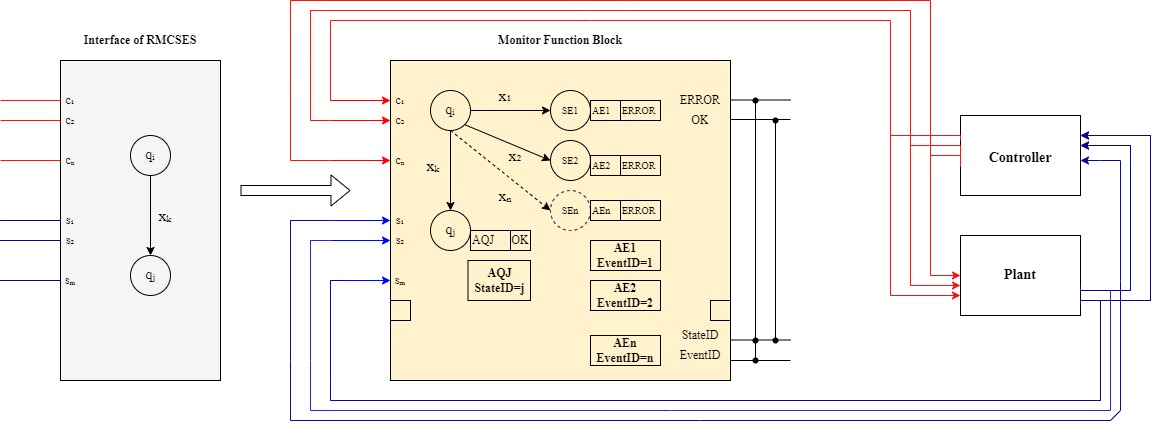
\includegraphics[width=1\textwidth]{chapters/images/chapter4/ConformaceCheckingApp.jpg}
	\caption{Application for conformance checking. The structure shows a closed-loop system consisting of a plant and controller, with the RMCSES (Reference Model of Control/Sensor Events Sequencing) connected for conformance checking. The monitor function block receives input signals from both controller and sensor components and generates OK/ERROR outputs based on conformance to the reference model.}
	\label{conformanceCheckingApp}
\end{figure*}

The structure of the application for conformance checking is depicted in Figure \ref{conformanceCheckingApp}. The application is based on a closed-loop system that includes a plant and a controller. The RMCSES obtained from the event log is connected to the closed-loop system for the purpose of conformance checking. The RMCSES is implemented as a finite state machine that uses input data to drive its logic. The monitor function block is capable of detecting errors and verifying the correct sequence of steps in the process flow by monitoring events from sensors and actuators in real time. When the monitor detects a valid transition, it generates an "OK" output indicating successful operation. If an unexpected event occurs, it transitions to an error state and produces an "ERROR" event with details about the event that caused the error.

The transformation from finite state machines to monitor ECCs follows a systematic algorithmic approach that ensures complete coverage of all possible system states and transitions. This transformation is essential for implementing real-time monitoring capabilities in industrial control systems. The algorithm takes a finite state machine representing the expected system behavior and produces an ECC with comprehensive error handling capabilities.

Algorithm \ref{FSMtoMonitor} provides the formal description of this transformation process, which involves creating both conforming and non-conforming ECC transitions. The algorithm operates in two main phases: first, it creates conforming ECC transitions that represent valid system behavior, generating "OK" outputs when expected events occur. Second, it creates non-conforming ECC transitions that capture all possible error scenarios, generating "ERROR" outputs with detailed information about the specific event and state where the error occurred.

\begin{algorithm}[T]
    \caption{FSM to Monitor ECC }
    \label{FSMtoMonitor}
\SetKwInOut{Input}{Input}
\SetKwInOut{Output}{Output}

\Input{ FSM = \{ Q: $\{q_0, q_1, \ldots, q_{n-1}\}$  
is a set of \\ states, where  $q_0$ is an initial state;\\
CS:  $\{X_1, X_2, \ldots, X_{p+r}\}$ 
is a set of input \\ symbols, where $X_i \in C \cup S$, where \\ C= $\{c_1,c_2,..., c_p\}$ is a set of control \\ signals, and S= $\{s_1,s_2,..., s_r\}$ is a set of \\ sensor signals; \\
$\delta \subseteq Q \times CS \times Q$ \} is a transition relation;
}
\Output{ ECC = \{ QC: $\{q_0, q_1, \ldots, q_{n-1}, {SE_n, SE_{n+1}} \dots {SE_{n+p+r-1}}\} \supset Q $ 
is a set of ECC states; \\
CS is a set of input events (see above);\\
Out: $\{\text{OK}, \text{ERROR}\}$  is a set of output events;\\
Alg= $\{a_0, a_1, \ldots, a_{n+p+r-1} \} $ is a set of \\ algorithms; \\ 
$\phi: \{ \text{Q} \times \text{CS} \rightarrow \text{QC} \times \text{Alg} \times \text{Out}$ \}  is an \\ ECC  transition function\} 

}
StateID=$q_0$  \\
{/* Creating the conforming (right) ECC transitions */}

\ForEach{$(q_i, X_k, q_j) \in \delta$ }{ 
Create ECC Transitions:
$(q_i, X_k) \rightarrow ( q_j, a_j, \text{OK})$
$a_j.StateID=j$  
} 

{/* Creating the non-conforming (erroneous) ECC transitions */}

\ForEach{$ q_w \in Q$ }{ 
\ForEach{$ X_e \in CS$ - $T(q_w)$}{ 
Create ECC Transitions:
$(q_w, X_e) \rightarrow (SE_e, a_e, \text{ERROR})$
$a_e.EventID=e$  
} 
} 
\Return{ECC}\; 

\textbf{ *Note* : Used variables and sets} \\

 StateID is an  output variable of the FB Monitor that stores the identifier of the current ECC  state;  \\

$a_j$.StateID is an occurrence of the  StateID  variable in the $a_j$ algorithm  associated with an ECC state;   \\

EventID is an  output variable of the FB Monitor that stores the identifier of the erroneous (not expected) input event; \\

$a_e$.EventID is an  occurrence of the EventID variable in the $a_e$ algorithm associated with an ECC state; \\

$T(q_w) \subseteq CS$ is a set of signals labelling the transitions outgoing from the ECC state $q_w \in Q$.

\end{algorithm}

The monitor implementation provides several key advantages for industrial control systems. First, it offers real-time error detection with immediate feedback on system state and error conditions. Second, it maintains detailed error information including both the state where the error occurred (StateID) and the specific event that caused the error (EventID). Third, it ensures complete coverage of all possible input events from each state, guaranteeing that any deviation from expected behavior will be detected. This comprehensive monitoring capability is essential for safety-critical applications where early detection of system malfunctions can prevent equipment damage and ensure operational safety.

The monitor continues operation until the first error is detected, after which it becomes non-responsive to prevent further processing. This behavior ensures that the system can be immediately stopped when a deviation is detected, preventing cascading failures and maintaining system integrity. The detailed error information provided by the monitor enables rapid diagnosis and correction of system issues, significantly reducing downtime and improving system reliability.

\section{Interactive Learning for Automatic Controller Generation}

The development of control logic for industrial automation systems traditionally requires significant domain expertise and manual programming effort. The interactive learning approach addresses this challenge by leveraging process mining techniques to automatically generate controllers from recorded behavioral traces, significantly reducing development time and improving system reliability.

\subsection{Simulation-Based Event Recording}

The foundation of interactive learning lies in the systematic recording of system behavior through simulation models. This approach uses 3D simulation environments, such as Visual Components, to create virtual representations of industrial systems that can be manipulated and observed without the risks and costs associated with physical experimentation.

The simulation environment provides a controlled setting where actuator signals can be manually triggered in appropriate sequences to generate desired process scenarios. Each interaction with the simulation model produces events that are recorded in chronological order, creating comprehensive behavioral traces that capture the complete system dynamics. This approach enables the generation of diverse process scenarios that might be difficult or dangerous to create in physical systems.



The recorded event logs capture the complete interaction between the simulation model and the operator, including sensor readings, actuator commands, and system state information. This comprehensive data collection ensures that the generated control logic accurately reflects the intended system behavior and can handle the full range of operational scenarios.

The simulation-based approach offers several advantages over traditional controller development methods. First, it eliminates the need for extensive domain knowledge in control system design, as the controller logic emerges directly from the recorded behavior. Second, it reduces development time by automating the transformation from behavioral requirements to executable control code. Third, it improves system reliability by ensuring that the controller logic is consistent with the observed system behavior.

\subsection{Process Discovery and Petri Net Generation}

The transformation from recorded event logs to executable control logic involves several systematic steps, beginning with process discovery to extract formal models from the behavioral traces. The alpha algorithm serves as the primary process discovery method, generating Petri nets that represent the system's behavioral patterns in a mathematically rigorous format.

The generated Petri nets capture the causal relationships between events, representing the system's state transitions and control flow. These models provide a formal foundation for understanding system behavior and serve as the basis for controller generation. The Petri net representation is particularly valuable because it can handle concurrent activities, sequential dependencies, and complex synchronization requirements that are common in industrial automation systems.


The Petri net generation process includes several important considerations. First, the addition of supplementary transitions, such as "Repeat" transitions, enables cyclic operation that is typical in manufacturing processes. Second, the stepwise simulation of the Petri net validates the model's correctness and ensures that it accurately represents the intended system behavior. Third, the conversion to reachability graphs provides a finite state machine representation that can be directly implemented in control systems.

The reachability graph represents all possible states and transitions of the system, providing a complete behavioral model that can be analyzed for properties such as deadlock freedom, liveness, and reachability. This analysis ensures that the generated controller will behave correctly under all operational conditions and can handle unexpected situations gracefully.

\subsection{Transformation to IEC 61499 Function Blocks}

The final step in the interactive learning process involves transforming the formal process models into executable IEC 61499 function blocks. This transformation requires careful mapping between the mathematical representation of the Petri net and the practical implementation requirements of industrial control systems.

The transformation process begins with the conversion of the reachability graph to a deterministic finite state machine (FSM). This conversion involves handling non-deterministic transitions, often represented as spontaneous or lambda transitions in the original Petri net. The determinization process ensures that the resulting FSM has unique transitions for each input combination, making it suitable for implementation in control systems.


The transformation from FSM to IEC 61499 function blocks involves several key steps. First, the FSM states are mapped to ECC states in the function block. Second, the FSM transitions are converted to ECC transitions with appropriate conditions and actions. Third, the input and output events are defined based on the sensor and actuator signals identified in the original event log.

The resulting function block interface includes input events for all sensor signals and output events for all actuator signals. The ECC implements the control logic by defining state transitions that respond to sensor inputs and generate appropriate actuator outputs. This implementation ensures that the generated controller behaves exactly as recorded during the interactive learning process.


The interactive learning approach provides several significant advantages for controller development. First, it reduces development time by automating the transformation from behavioral requirements to executable code. Second, it improves system reliability by ensuring that the controller logic is consistent with observed system behavior. Third, it enables rapid prototyping and testing of different control strategies without extensive programming effort.

\section{Automatic Plant Model Generation and Real-Time Monitoring}

The extension of process mining techniques to automatic plant model generation represents a significant advancement in formal verification capabilities for industrial control systems. This approach addresses the critical challenge of creating accurate plant models for closed-loop system verification, enabling comprehensive analysis of system behavior and real-time monitoring of operational compliance.

\subsection{Reference Model of Control/Sensor Events Sequencing}

The foundation of automatic plant model generation lies in the Reference Model of Control/Sensor Events Sequencing (RMCSES), a formal model that represents the complete behavior of a closed-loop industrial automation system. This model is derived from process mining of event logs recorded during error-free system operation over extended periods.

The RMCSES provides a condensed representation of vast event logs, encompassing all possible signals from all system components. Conceptually, if the event log represents a collection of sentences describing system behavior, then RMCSES functions as a sentence generator for this formal language. This representation enables the model to be readily implemented in software or hardware, making it suitable for real-time applications.

The RMCSES interface focuses exclusively on control signals originating from the controller and informative signals originating from sensors, representing the interface between the controller and the plant. Internal signals circulating within the control system and plant are not considered, though control signals from external sources such as operators can be included. This focus on the controller-plant interface makes the model particularly suitable for closed-loop system analysis and verification.

The model assumes that each component in the system operates in a cyclical, meaningful, and locally complete manner. Components are considered to have meaningful behavior when they have specific goals and actively work toward achieving them. Each component follows specific scenarios that begin with initialization and end with termination, with multi-functional devices potentially executing different scenarios depending on their current task or operation.

\subsection{Petri Net Decomposition and State Machine Generation}

The transformation from event logs to plant models involves several sophisticated steps, beginning with Petri net construction and proceeding through decomposition and state machine generation. This process addresses the complexity of industrial systems by breaking down complex behaviors into manageable components while preserving essential behavioral characteristics.

The Petri net decomposition process utilizes reachability graph methods to identify subsets of states and transitions, facilitating the partitioning of complex Petri nets into manageable modules. This approach provides a structured and systematic method for exploring all reachable states and transitions within the system, ensuring completeness in capturing all potential behaviors.

The reachability graph method, while comprehensive, can suffer from state space explosion in complex systems. To address this challenge, several strategies are employed: state space reduction using symbolic representations such as Binary Decision Diagrams (BDDs), abstraction and aggregation methods that focus on essential behavioral properties, partial order reduction techniques that avoid redundant interleavings, and on-the-fly exploration that generates states as needed.

The composition of State Machine Components (SMCs) into a cohesive FSM requires careful integration to ensure synchronization and coordination. Parallel composition and synchronization techniques are preferred for IEC 61499 systems, as they align with the distributed and modular architecture of these systems. This approach enables concurrent execution of SMCs while maintaining proper coordination and communication between distributed components.

\subsection{Plant Model Transformation and Implementation}

The transformation from finite state machines to plant model ECCs represents a critical step in the automatic plant model generation process. This transformation requires careful handling of the different types of signals and transitions that characterize plant behavior in industrial control systems.

\begin{figure*}[!t]
	\centering
	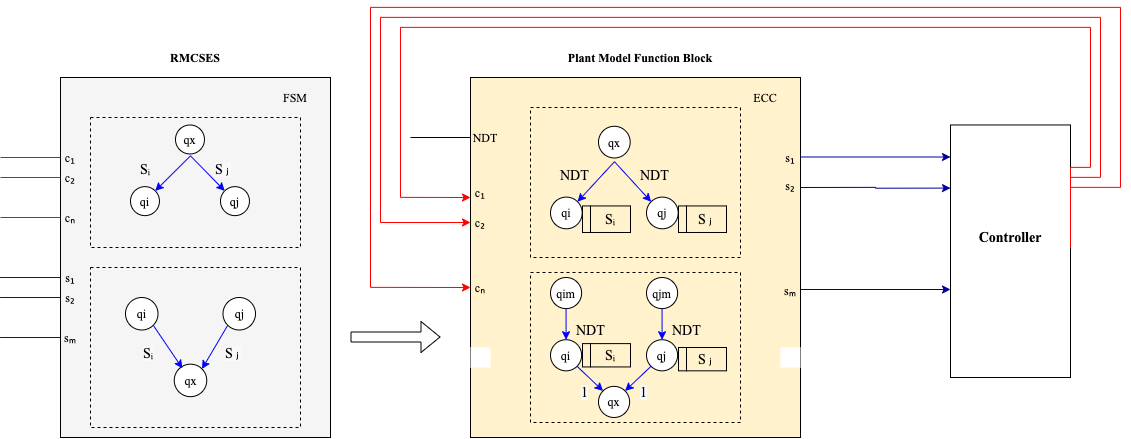
\includegraphics[width=0.9\textwidth]{chapters/images/chapter4/VerificationApp1.png}
	\caption{Application for verification. The structure shows a closed-loop system formed by connecting a plant model obtained from the RMCSES with either a new or existing controller. The plant model interface comprises control signals and non-deterministic transitions (NDT) as input signals, while sensor signals are designated as output signals. This configuration enables formal verification using tools such as NuSMV with CTL/LTL specifications.}
	\label{verificationApp}
\end{figure*}

The presented application for verification follows a structure illustrated in Figure \ref{verificationApp}, where a closed-loop system is formed by connecting a plant model obtained from the RMCSES with either a new or an existing controller. An existing controller is utilized to construct the RMCSES, whereas a new controller is connected with RMCSES for the purpose of verification. The verification process involves conformance checking to ensure that the newly developed controller operates in accordance with the previous controller. The plant model interface comprises control signals and non-deterministic transitions (NDT) as input signals, while sensor signals are designated as output signals. This configuration enables formal verification using tools such as NuSMV with CTL/LTL specifications.

The transformation from RMCSES to plant model involves specific rules for handling sensor and control signals. Transitions triggered by sensor signals are replaced with non-deterministic transitions (NDT) that can fire at arbitrary time intervals, with the output of the next state serving as a sensor event signal. Control signal transitions remain unchanged, as the plant should respond directly to control inputs. This transformation ensures that the plant model accurately represents the uncontrolled behavior of the physical system while maintaining compatibility with formal verification tools.

The transformation process follows a systematic algorithmic approach that handles the complexity of plant behavior modeling. This transformation is essential for creating accurate plant models that can be used for formal verification and closed-loop system analysis. The algorithm takes a finite state machine representing the overall system behavior and produces a plant model ECC that accurately represents the uncontrolled plant behavior.

Algorithm \ref{FSMtoPlant} provides the formal description of this transformation process, which involves processing control signals, sensor signals, and handling converging sensor signals through the introduction of intermediate states. The algorithm operates in three main phases: first, it processes control signal transitions, maintaining them unchanged as the plant should respond directly to control inputs. Second, it processes sensor signal transitions that are not converged, replacing them with non-deterministic transitions (NDT) that can fire at arbitrary time intervals. Third, it handles converging sensor signals by introducing intermediate states that produce appropriate sensor signals before converging to the target state.

\begin{algorithm}[t!]
    \caption{FSM to Plant model ECC }
    \label{FSMtoPlant}
\SetKwInOut{Input}{Input}
\SetKwInOut{Output}{Output}

\Input{ FSM = \{ Q: $\{q_0, q_1, \ldots, q_{n-1}\}$ \\
is a set of states, where $q_0$ is an initial state; \\
CS =  $ C \cup S$ is a set of input signals, where \\  C = $\{c_1, c_2, \ldots, c_p \}$ is a set of control \\  signals, \\  S = $\{s_1, s_2 \ldots, s_r \}$ is a set of sensorsignals; \\
$\delta \subseteq Q \times CS \times Q$ is a transition  relation; \}
}
\Output{ ECC = \{ $QC= Q \cup D$ is a set of ECC states, where D is a set of additional ECC states created dynamically;
$Cond= TC \cup \{1\}$ is a set of ECC transition  conditions, where $TC= C \cup \{NDT\}$ is a set  of input events;
S is a set of output events (see above);\\
$ \phi: QC \times Cond \rightarrow QC \cup QC\times S $ \\ is an ECC  transition function
\}
}

/* Processing the FSM transition labelled by control signals */

\ForEach{$(q_i, \sigma, q_j) \in \delta$}{
    \If{$\sigma \in $ C}{
        Create ECC Transition:
        $(q_i,  \sigma ) \rightarrow (q_j)$;\
    }
}
/* Processing the FSM transition labelled by sensor signals which are not converged */

\ForEach{$(q_i, \sigma, q_j) \in \delta$}{
    \If{$\sigma \in  S $ \text{AND}  $q_i \notin QJ$}{
        Create ECC Transition:
        $(q_i,  NDT ) \rightarrow (q_j, \sigma)$;\
    }
}

/* Processing the FSM transition labelled by converging sensor signals */

\ForEach{$(q_w \in QJ) $}{
\ForEach{$(q_i, \sigma, q_w) \in \delta'}{
    \If{$\sigma \in  S $}{
        Create ECC State $d \in D$ \\
        Create ECC Transition:
    $(q_i,  NDT ) \rightarrow (d, \sigma)$ ; \ \\
        $(d,  1 ) \rightarrow (q_w)$ ;\
    }
}

}
    \Return{ECC}\;

\textbf{ *Note* : Used variables and sets} \\
\BlankLine

$QJ= { \{ q_j \in Q , | \{(q_i, s_k, q_j) \in \delta'\}|>1} \} $, where $\delta' = \delta \cap  Q \times S \times Q$ is a set of ECC states which have converging sensor signals in the FSM

\end{algorithm}

The plant model implementation addresses several important challenges in industrial control system modeling. First, it handles diverging sensor signals by creating separate NDT transitions for each possible sensor output, ensuring that all possible plant behaviors are captured. Second, it manages converging sensor signals by introducing intermediate states that produce appropriate sensor signals before converging to the target state, maintaining the non-deterministic nature of plant behavior. Third, it maintains the non-deterministic nature of plant behavior while providing a deterministic interface for integration with control systems, enabling formal verification using tools such as NuSMV and CTL/LTL specifications.

This algorithmic approach ensures that the generated plant model accurately represents the uncontrolled behavior of the physical system while maintaining compatibility with formal verification tools. The plant model can be used for formal verification using tools such as NuSMV and CTL/LTL specifications, enabling comprehensive analysis of system properties including safety, liveness, and reachability. This verification capability is particularly valuable for safety-critical applications where formal guarantees of system behavior are required.

\subsection{Monitor Implementation for Real-Time Conformance Checking}

The automatic generation of monitors represents a critical application of the RMCSES, enabling real-time detection of deviations from expected system behavior. These monitors are implemented as IEC 61499 function blocks that can be deployed in operational systems to provide continuous monitoring and early warning of potential issues.

The monitor implementation involves transforming the RMCSES into a function block that receives input signals from both controller and sensor components. The monitor's ECC is generated using transformation rules that map FSM states and transitions to appropriate ECC states and transitions. When the monitor detects a valid transition, it generates an "OK" output indicating successful operation. If an unexpected event occurs, the monitor transitions to an error state and produces an "ERROR" event with details about the event that caused the error.

The monitor's error detection capabilities are comprehensive, covering all possible input events from each state. For each state in the FSM, the monitor defines transitions to error states for all input events that are not specified in the reference model. This complete coverage ensures that any deviation from expected behavior is detected immediately, providing robust protection against system malfunctions and unauthorized operations.

The monitor implementation includes several important features. First, it provides detailed error information including the state where the error occurred and the specific event that caused the error. Second, it continues operation until the first error is detected, after which it becomes non-responsive to prevent further processing. Third, it can be easily integrated with existing control systems without requiring significant modifications to the operational infrastructure.

\subsection{Plant Model Generation for Formal Verification}

The automatic generation of plant models extends the capabilities of process mining to formal verification applications. These plant models represent the uncontrolled behavior of the physical system and can be integrated with control models to create complete closed-loop system representations suitable for formal analysis.

The plant model generation process involves extracting the uncontrolled plant behavior from the overall system model represented by the RMCSES. This extraction requires careful analysis to distinguish between control-driven and sensor-driven transitions, as the plant model should only respond to control signals and generate sensor signals based on its internal state.

The transformation from FSM to plant model involves specific rules for handling sensor and control signals. Transitions triggered by sensor signals are replaced with non-deterministic transitions (NDT) that can fire at arbitrary time intervals, with the output of the next state serving as a sensor event signal. Control signal transitions remain unchanged, as the plant should respond directly to control inputs.

The plant model implementation addresses several important challenges. First, it handles diverging sensor signals by creating separate NDT transitions for each possible sensor output. Second, it manages converging sensor signals by introducing intermediate states that produce appropriate sensor signals before converging to the target state. Third, it maintains the non-deterministic nature of plant behavior while providing a deterministic interface for integration with control systems.

The generated plant model can be used for formal verification using tools such as NuSMV and CTL/LTL specifications. The model can be converted to SMV format using the fb2smv tool, enabling comprehensive analysis of system properties including safety, liveness, and reachability. This verification capability is particularly valuable for safety-critical applications where formal guarantees of system behavior are required.

\section{Integration and Applications}

The three approaches presented in this chapter represent complementary aspects of process mining applications in industrial control systems, each addressing different challenges in system understanding, control generation, and verification. Their integration provides a comprehensive framework for addressing the complex requirements of modern industrial automation.

\subsection{Comprehensive System Analysis Framework}

The integration of process model extraction, interactive learning, and automatic plant model generation creates a comprehensive framework for industrial control system analysis and development. This framework enables end-to-end system understanding, from initial behavior recording through formal verification and operational monitoring.

The framework begins with process model extraction, which provides fundamental understanding of system behavior through analysis of recorded event logs. This understanding serves as the foundation for both controller generation and plant model development, ensuring consistency across all system representations.

Interactive learning builds upon this foundation by enabling automatic controller generation from recorded behavioral traces. This approach reduces development time and improves system reliability by ensuring that control logic is consistent with observed system behavior. The generated controllers can be immediately deployed or used as starting points for further refinement.

Automatic plant model generation extends the framework to formal verification applications, enabling comprehensive analysis of closed-loop system behavior. The generated plant models can be used with existing or newly developed controllers to verify system properties and ensure compliance with safety and performance requirements.

\subsection{Industrial Applications and Case Studies}

The presented approaches have been validated through several industrial case studies, demonstrating their effectiveness in real-world applications. The gripper and conveyor system case study illustrates the application of process model extraction for system understanding and anomaly detection. This case study shows how process mining can be used to analyze complex manufacturing processes and identify potential improvements in system operation.

The interactive learning case study demonstrates the application of simulation-based controller generation for a production system with multiple components including conveyors, grippers, and autonomous guided vehicles. This case study shows how the approach can handle complex, multi-component systems and generate controllers that accurately reflect desired system behavior.

The pneumatic cylinder case study illustrates the application of automatic plant model generation and real-time monitoring. This case study shows how the approach can be used for formal verification of safety-critical systems and real-time monitoring of operational compliance.

\begin{figure*}[!t]
	\centering
	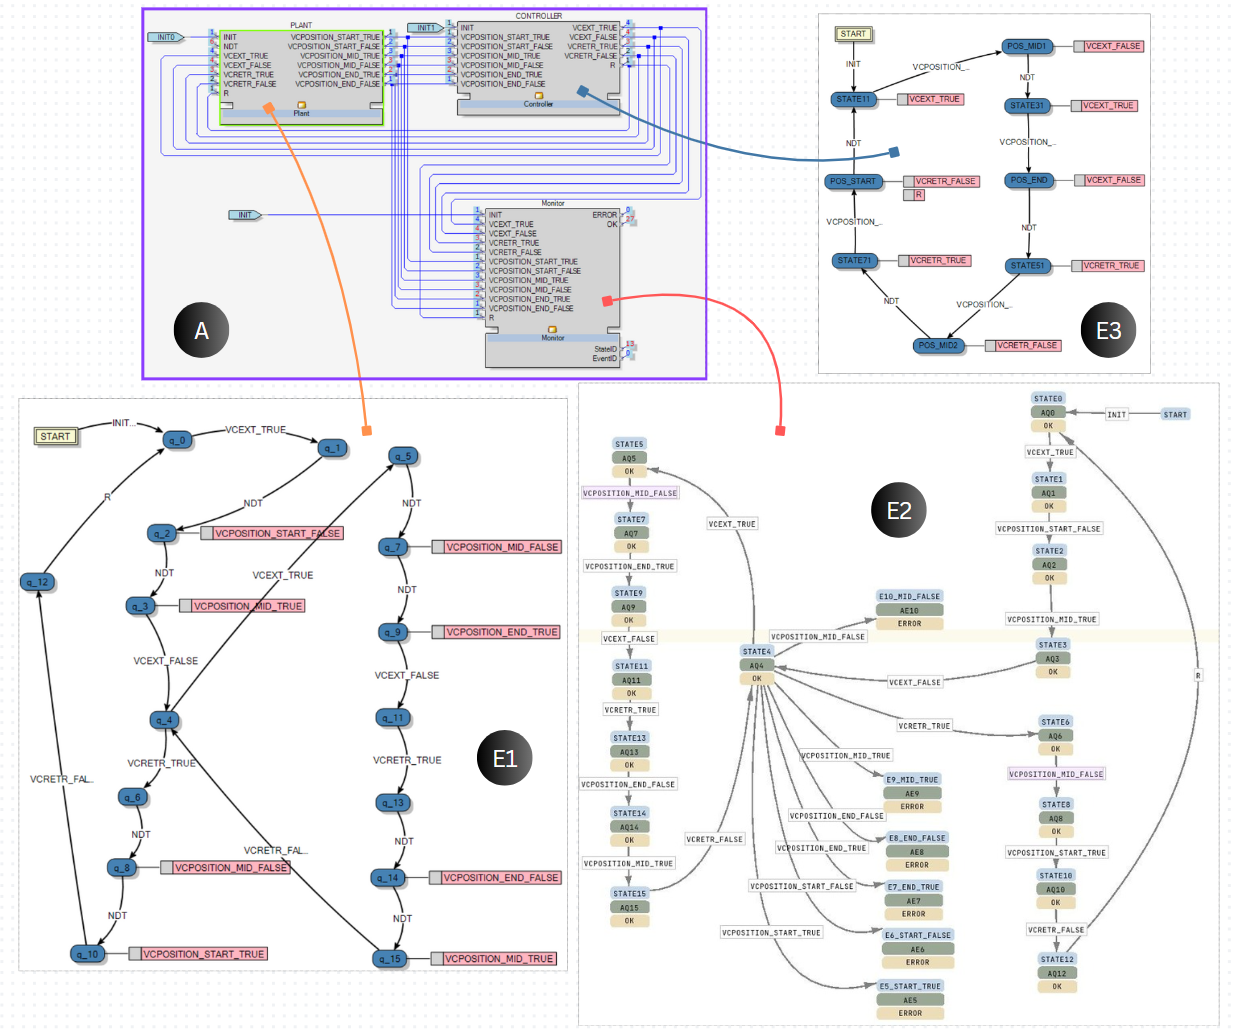
\includegraphics[width=1\textwidth]{chapters/images/chapter4/CLMC.PNG}
	\caption{Closed-loop system of plant and controller model with the monitor. The figure shows the integration of a plant model, controller, and monitor in a closed-loop configuration. The monitor function block receives input signals from both controller and sensor components, generating OK/ERROR outputs based on conformance to the reference model. The ECC diagrams illustrate the internal logic of both the plant model and monitor function blocks.}
	\label{CL_plant_controller_monitor}
\end{figure*}

Figure \ref{CL_plant_controller_monitor} illustrates a practical implementation of the closed-loop system integration with monitor for a pneumatic cylinder case study. The system consists of a plant model, controller, and monitor connected in a closed-loop configuration. The monitor function block receives input signals from both controller and sensor components, generating OK/ERROR outputs based on conformance to the reference model. The Execution Control Chart (ECC) diagrams show the internal logic of both the plant model and monitor function blocks, demonstrating how the transformation from finite state machines to IEC 61499 function blocks is implemented in practice.

In this implementation, the monitor generates an 'OK' event with the corresponding StateID when the system process executes in the correct order. In the case of any deviation from the expected process behavior, an 'ERROR' signal is emitted along with the 'EventID' indicating the specific event responsible for the deviation. The monitor continues operation until the first error is detected, after which it becomes non-responsive to prevent further processing. This real-time monitoring capability is essential for ensuring system safety and reliability in industrial applications.

These case studies demonstrate the versatility of the presented approaches and their applicability to a wide range of industrial applications. The approaches can be adapted to different system types, from simple single-component systems to complex multi-component manufacturing lines, providing flexible solutions for various industrial automation challenges.

\subsection{Future Research Directions}

The integration of process mining with industrial control systems opens several promising research directions that could further enhance the capabilities and applicability of these approaches.

First, the development of more sophisticated process discovery algorithms could improve the quality and accuracy of generated models. Current algorithms may struggle with complex, highly concurrent systems or systems with significant noise in their event logs. Advanced algorithms that can handle these challenges would expand the applicability of the approaches to a broader range of industrial systems.

Second, the integration of machine learning techniques with process mining could enable adaptive models that improve over time based on new observations. This capability would be particularly valuable for systems that evolve or change their behavior over time, enabling continuous improvement of system understanding and control.

Third, the development of more efficient algorithms for handling large-scale event logs could enable the application of these approaches to complex, multi-facility manufacturing systems. Current approaches may face computational challenges when dealing with very large event logs or complex system architectures.

Fourth, the integration of these approaches with emerging technologies such as digital twins and edge computing could enable real-time process mining and control generation. This integration would enable dynamic adaptation of control systems based on real-time analysis of system behavior, providing more responsive and adaptive automation solutions.

The research presented in this chapter demonstrates the significant potential of process mining techniques for addressing critical challenges in industrial control systems. The three complementary approaches provide comprehensive solutions for system understanding, control generation, and verification, while the integration of these approaches creates a powerful framework for industrial automation development and analysis.

As industrial systems become increasingly complex and interconnected, the need for automated methods for system understanding and control generation will continue to grow. The approaches presented in this chapter provide a solid foundation for addressing these challenges and enable the development of more intelligent, adaptive, and reliable industrial automation systems.

The future of industrial automation lies in the integration of data-driven approaches with formal methods, creating systems that can learn from their environment, adapt to changing requirements, and provide formal guarantees of their behavior. The process mining approaches presented in this chapter represent important steps toward this vision, providing practical methods for realizing intelligent industrial automation systems that can meet the demands of modern manufacturing.
